\section{Results}
\label{sec:results}

\subsection{Target shrinkage does not guarantee learnability}
\label{sec:reference-correction}

To examine whether target shrinkage and model-relative learnability are equivalent, we first test a standard target-preprocessing protocol used in machine-learning interatomic potentials (MLIPs) \cite{tran2023oc22,schutt2023schnetpack2,pelaez2024torchmdnet2}. These reference corrections are widely used to improve optimization and training stability. First, fixed element-wise atomic references are subtracted from the total DFT energy to yield the reference-corrected energy, \(E_{\rm ref}\). Next, a linear Bag-of-Elements (BoE) model fitted to elemental counts is subtracted, defining the residual target:

\begin{equation}
E_{\rm ref,BoE}=E_{\rm ref}-E_{\rm BoE}.
\label{eq:boe-reference-correction}
\end{equation}

Because the subtracted references are added back at inference, this procedure constitutes stacked delta learning. The MAE of the residual prediction is exactly equal to that of the complete stacked prediction (SI Section~1).

\begin{figure}[H]
  \centering
  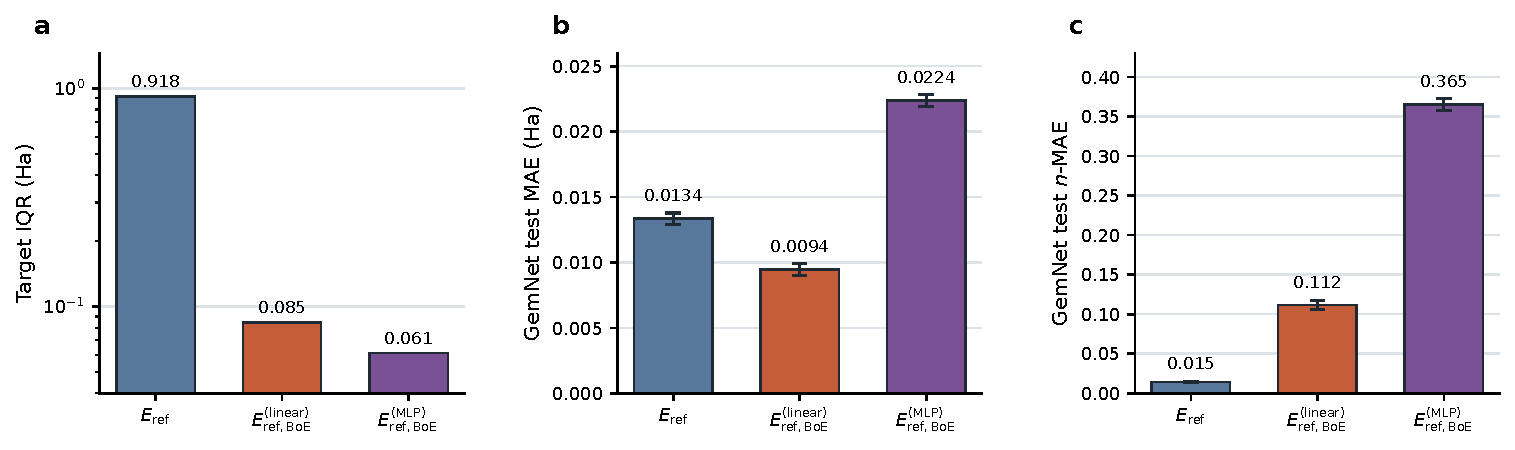
\includegraphics[width=\linewidth]{fig01_reference_correction}
  \caption{\textbf{Target scale and GemNet accuracy after BoE correction.} \textbf{a,} Test-set IQR for \(E_{\rm ref}\) and its linear- and MLP-BoE residuals. \textbf{b,} Mean GemNet test MAE. \textbf{c,} Normalized MAE, \(n\text{-MAE}_{\rm test}=\operatorname{MAE}_{\rm test}/\operatorname{IQR}_{\rm test}(y)\). Error bars show sample standard deviations across three seeds.}
  \label{fig:reference-correction}
\end{figure}

In addition to its conventional role in improving optimization and training stability, linear BoE correction reduces the mean tmQM test MAE by a factor of \(1.41\) (Fig.~\ref{fig:reference-correction}b). BoE correction is therefore a successful form of delta learning. However, this improvement could arise either from target shrinkage or from a transformation that makes the residual better aligned with GemNet's inductive bias and, consequently, easier to learn relative to its scale.

To distinguish these effects, we use the normalized MAE, \(n\text{-MAE}_{\rm test}=\operatorname{MAE}_{\rm test}/\operatorname{IQR}_{\rm test}(y)\), where the interquartile range (IQR) measures the central scale of the test target. The \(n\)-MAE provides an empirical, model-dependent measure of learning difficulty after accounting for target scale. Under a pure rescaling, MAE and IQR change by the same factor, leaving \(n\)-MAE unchanged. An algebraic rescaling control confirms this invariance (SI Note~2). An increase in \(n\)-MAE after a target transformation therefore indicates that the transformed target is harder for the same model to learn relative to its own scale, whereas a decrease indicates improved model-relative learnability.

For linear BoE correction, the \(n\)-MAE of \(E_{\rm ref,BoE}\) is \(7.7\)-fold larger than that of \(E_{\rm ref}\) (Fig.~\ref{fig:reference-correction}c), while the target IQR decreases by a factor of \(10.9\) (Fig.~\ref{fig:reference-correction}a). The reduction in absolute MAE therefore does not result from improved model-relative learnability. Instead, the substantial target shrinkage outweighs the increase in normalized learning difficulty.

The linear BoE result demonstrated that substantial target shrinkage can improve absolute performance despite reducing normalized learnability. To test whether further target shrinkage continues to improve downstream performance, we replace linear BoE with a nonlinear MLP fitted to the same elemental-count inputs. This control increases baseline flexibility while holding its input information fixed. The MLP residual is \(1.38\)-fold smaller by IQR, but its \(n\)-MAE is \(3.27\)-fold larger, resulting in a \(2.37\)-fold increase in absolute MAE (Fig.~\ref{fig:reference-correction}). SchNet shows the same trend (SI Section~1). This result rejects the assumption that progressively removing more target variation necessarily produces progressively better residual learning.

These results establish the central problem addressed in this work: baseline accuracy and its accompanying residual scale reduction alone cannot predetermine the success of a target transformation. While the normalized error assesses scale-independent learnability of the target, it remains a post-hoc metric only available after training. A practical target-design strategy therefore requires a pre-training measure that estimates how a baseline transformation changes the normalized learnability of its residual.

\subsection{Pre-training roughness quantifies model-relative learnability}
\label{sec:pretraining-roughness}

To evaluate whether a baseline residual will be learnable downstream, we measure its smoothness relative to structural information accessible to the target neural network. However, because the trained internal representations of message-passing networks such as SchNet and GemNet are learned during optimization, they are unavailable \textit{a priori}. We address this by constructing fixed, explicit geometric feature spaces, termed \textbf{representation proxies}, that approximate the geometric information available to each architecture:

\begin{itemize}
  \item \textbf{Pair-Radial Expansion (PRE):} a two-body feature space that expands element-resolved pairwise interatomic distances, \(r_{ij}\), using Gaussian radial basis functions up to a local spatial cutoff. By capturing distance distributions without explicit angular information, PRE serves as a representation proxy for pairwise message-passing architectures such as SchNet.
  \item \textbf{PRE with angular terms (PRE+A):} an extended three-body feature space that augments PRE with central-element-resolved triplet angle distributions, \(\theta_{ijk}\). By capturing angular geometry in addition to pairwise distances, PRE+A serves as a proxy for directional, triplet-based architectures such as GemNet.
\end{itemize}

Detailed descriptor formulations, radial basis dimensions, and hyperparameter choices are provided in Methods (Sections~\ref{sec:methods-baselines} and~\ref{sec:methods-roughness-diagnostics}) and SI Methods.

By mapping molecules into these proxy feature spaces, we can evaluate target variation before model optimization. We construct a \(k\)-nearest-neighbour graph connecting test molecules with similar standardized descriptor vectors. Edge weights, \(w_{ij}\), encode feature-space similarity through a locally scaled Gaussian kernel of cosine distance:
\begin{equation}
  w_{ij}=\exp\!\left(-\frac{d_{ij}^{2}}{\sigma_i\sigma_j}\right),
  \label{eq:dirichlet-edge-weight}
\end{equation}
Here, \(d_{ij}\) is the cosine distance between standardized descriptor vectors for molecules \(i\) and \(j\), and \(\sigma_i\) is a local distance scale, defined as the distance from molecule \(i\) to its \(k\)-th nearest neighbour.

Using these edge weights, we quantify target variation through the IQR-normalized graph Dirichlet roughness, \(D_{\rm IQR}\) \cite{belkin2006manifold}:
\begin{equation}
  D_{\rm IQR}(y)=\frac{1}{\sum_{\{i,j\}\in\mathcal E}w_{ij}}
  \sum_{\{i,j\}\in\mathcal E}
  w_{ij}\frac{(y_i-y_j)^2}{\operatorname{IQR}_{\rm test}(y)^2}.
  \label{eq:dirichlet-roughness}
\end{equation}
Here, \(\mathcal E\) is the set of unique undirected graph edges. For targets with nonzero IQR, this formulation normalizes local squared target differences by the squared central target spread, making \(D_{\rm IQR}\) invariant to nonzero uniform target rescaling. A lower value indicates that molecules with similar proxy descriptors have similar target labels relative to this central spread. This provides an architecture-informed, pre-training diagnostic for assessing residual learnability without first training a downstream GNN; its predictive value is tested in the following comparisons.

Applying this normalized roughness metric to the composition-corrected energy targets, we find that \(D_{\rm IQR}\) increases from \(0.548\) for \(E_{\rm ref}\) to \(1.127\) for linear-BoE and \(1.658\) for MLP-BoE. This ordering matches the post-training \(n\)-MAE ordering observed in Figure~\ref{fig:reference-correction}. The MLP-BoE residual is similarly rougher than linear-BoE in the SchNet-aligned PRE space (\(1.709\) versus \(1.152\); SI Note~6).

In the following sections, we further test whether \(D_{\rm IQR}\) can serve as a reliable qualitative ordering proxy for target roughness and whether that roughness describes the intrinsic learnability assessed post-training using \(n\)-MAE.

\subsection{Residual roughness guides target design beyond baseline accuracy}
\label{sec:residual-design}

To test whether \(D_{\rm IQR}\) reliably predicts downstream learnability, we systematically evaluated how different baseline physical approximations alter residual scale, roughness, and deep model performance. Our goal is to construct simple, computationally inexpensive baseline models that predict the atom- and composition-referenced DFT energy, \(E_{\rm ref,BoE}^{\rm DFT}\). Subtraction of these predictions, \(\widehat{E}_b\), yields the transformed residual target, \(\Delta^b\), on which the downstream GNN models are trained.

We compare three descriptor-based baselines, BoB, PRE, and PRE+A, that capture progressively richer structural information. Alongside these, we evaluate xTB as our primary semiempirical comparison and DFTB as a supporting control. Table~\ref{tab:baseline-models} summarizes the five approaches:

\begin{enumerate}
  \item \textbf{Bag-of-Bonds (BoB):} a simple global descriptor tracking RDKit-derived typed-bond counts to capture basic compositional and functional-group variation, rather than the Coulomb-matrix entries used in the conventional BoB descriptor.
  \item \textbf{Pair-Radial Expansion (PRE):} repurposing the pairwise geometric representation introduced in Section~\ref{sec:pretraining-roughness} as an explicit input descriptor to capture local two-body geometry.
  \item \textbf{PRE with angular terms (PRE+A):} repurposing the three-body geometric representation from Section~\ref{sec:pretraining-roughness} as an input descriptor to capture local pairwise and angular geometry.
  \item \textbf{Extended tight-binding (xTB):} a semiempirical quantum-mechanical baseline providing molecule-wide electronic-structure information beyond the local geometric cutoffs of the descriptors.
  \item \textbf{Density functional tight-binding (DFTB\(\dagger\)):} a second semiempirical quantum-mechanical baseline used to test whether the trends observed with xTB extend to another electronic-structure method.
\end{enumerate}

\begin{table}[H]
  \centering
  \caption{\textbf{Baseline models used for target transformation.}}
  \label{tab:baseline-models}
  \small
  \setlength{\tabcolsep}{4pt}
  \renewcommand{\arraystretch}{1.2}
  \begin{tabular}{@{}>{\raggedright\arraybackslash}p{0.12\linewidth}>{\raggedright\arraybackslash}p{0.25\linewidth}>{\raggedright\arraybackslash}p{0.19\linewidth}>{\raggedright\arraybackslash}p{0.38\linewidth}@{}}
    \toprule
    Baseline model & Input features & Fitting approach & Physical/representation target \\
    \midrule
    BoB & Typed-bond counts (\mbox{RDKit}) & Linear / MLP & Compositional and functional-group variation \\
    PRE & Pairwise distances (\(r_{ij}\)) & Linear / MLP & Local two-body geometry (SchNet proxy) \\
    PRE+A & Distances and angles (\(r_{ij},\theta_{ijk}\)) & Linear / MLP & Local three-body geometry (GemNet proxy) \\
    xTB & Atomic identities and molecular coordinates & Semiempirical QM & Non-local electronic and higher-order interactions \\
    DFTB\(\dagger\) & Atomic identities and molecular coordinates & Semiempirical QM & Molecule-wide electronic structure; supporting comparison with xTB \\
    \bottomrule
  \end{tabular}
\end{table}

For each descriptor (BoB, PRE, and PRE+A), we fit both a linear regression model and a nonlinear multilayer perceptron (MLP); the MLPs share a unified hidden architecture (Methods). This dual-fitting strategy enables two controlled evaluations: varying the input descriptor under a fixed MLP architecture assesses how baseline information content alters residual structure, while comparing linear and MLP fits within the same descriptor family isolates the effect of baseline fitting capacity. For each supervised baseline \(b\), the target residual is defined as:

\begin{equation}
\Delta^b=E_{\rm ref,BoE}^{\rm DFT}-\widehat{E}_b,
\label{eq:descriptor-delta}
\end{equation}

In parallel, we evaluate xTB to provide a physics-based baseline that accounts for non-local electronic interactions \cite{bannwarth2019gfn2xtb}. Its residual, \(\Delta^{\rm xTB}\), is computed after applying the same atom- and composition-referencing protocol:

\begin{equation}
\Delta^{\rm xTB}
=E_{\rm ref,BoE}^{\rm DFT}-E_{\rm ref,BoE}^{\rm xTB}.
\label{eq:xtb-delta}
\end{equation}

The DFTB residual is constructed in the same way, using the atom- and composition-referenced DFTB energy \cite{elstner1998sccdftb,hourahine2020dftbplus}. DFTB calculations failed for 362 neutral tmQM molecules, so this control uses the successful-calculation subset and one GNN seed per architecture. DFTB\(\dagger\) is shown in the main figures for comparison but excluded from pooled correlations and regression fits. Matched-subset comparisons and calculation details are provided in SI Note~8.

Comparing MLP baselines across descriptor families reveals a clear trade-off between target accuracy and learnability. Progressing from BoB to PRE and PRE+A progressively increases baseline accuracy and reduces residual magnitude (Fig.~\ref{fig:residual-design}a,c). Judged strictly by baseline accuracy or residual scale, PRE+A would appear to offer the optimal \(\Delta\)-learning target. However, our roughness analysis yields a different conclusion. Although these baselines reduce target IQR by factors of \(3.3\), \(4.2\), and \(4.7\), respectively, they increase representation-space target roughness (\(D_{\rm IQR}\)) by factors of \(3.3\), \(9.5\), and \(7.6\) within GemNet-aligned PRE+A space (Fig.~\ref{fig:residual-design}b). Consequently, these smaller residuals remain rougher, and none improves GemNet test MAE over direct training on \(E_{\rm ref,BoE}\).

\begin{figure}[t]
  \centering
  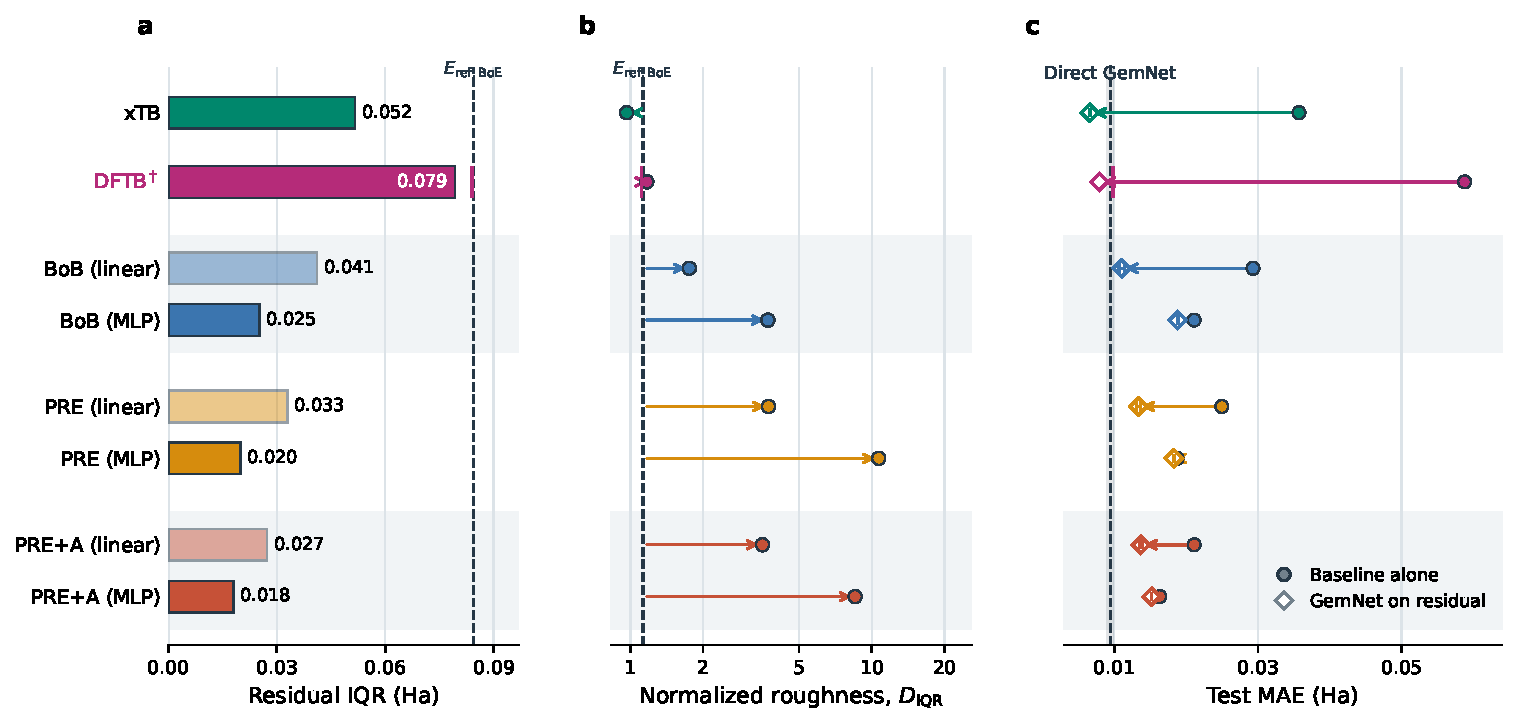
\includegraphics[width=\linewidth]{fig02_residual_design}
  \caption{\textbf{Baseline accuracy, residual roughness, and GemNet test performance.} \textbf{a,} Test residual IQR. \textbf{b,} Normalized roughness on the test PRE+A graph (log scale). \textbf{c,} Baseline-only test MAE (filled circles) and GemNet residual test MAE (open diamonds). Dashed lines mark the DFT-BoE parent or direct-GemNet reference; arrows show the corresponding changes. Main GNN results are three-seed means; error bars and shading show sample SD. Magenta DFTB\(^\dagger\) is a single-seed, valid-subset control, excluded from pooled analyses. Short magenta ticks mark its matched-subset parent references (SI Note~8).}
  \label{fig:residual-design}
\end{figure}

This degradation in learnability persists even when baseline input features remain fixed. Comparing linear and MLP fits within each descriptor family shows that increasing baseline expressivity consistently yields smaller yet rougher residuals, degrading GemNet test performance (Fig.~\ref{fig:residual-design}). For instance, transitioning from a linear to an MLP fit on BoB features reduces residual IQR by an additional factor of \(1.6\), yet GemNet test MAE increases \(1.7\)-fold. Thus, stripping away additional target variance without considering representation alignment can actively impede model generalization.

The poorer test performance on these rough residuals persists after normalization by test target IQR. For GemNet, the MLP-PRE residual has a normalized test error \(7.2\)-fold higher than the xTB residual. SchNet exhibits a similar discrepancy, with a \(4.9\)-fold difference (SI Note~6). Thus, even after accounting for target scale, the smaller MLP-PRE residual remains harder to predict on unseen structures.

In contrast, xTB leaves a larger residual than the BoB, PRE, and PRE+A baselines, yet GNNs trained on this residual achieve lower test errors. Among the primary baselines in Figure~\ref{fig:residual-design}, xTB is the only one that lowers both normalized roughness and GemNet test MAE: \(D_{\rm IQR}\) falls from \(1.127\) to \(0.964\), while mean test MAE falls from \(0.00945\) to \(0.00660\)~Ha. xTB therefore provides our primary evidence that smaller residuals are not necessarily easier for a GNN to learn.

DFTB provides a contrasting control on its valid subset: its residual is also relatively large, and has slightly higher roughness than the matched DFT parent in both PRE and PRE+A spaces. In PRE+A space, \(D_{\rm IQR}\) rises from \(1.113\) to \(1.169\), while the matched seed-101 GemNet test MAE falls from \(0.00979\) to \(0.00794\)~Ha (SI Note~8). DFTB remains a separate semiempirical control, not part of the pooled analysis. These results do not suggest that larger residuals are inherently better. Rather, they show that an effective baseline must leave a residual that the downstream model can learn, not simply one with a smaller magnitude.

\subsection{Model-relative target roughness predicts scale-normalized learnability}
\label{sec:roughness-predicts}

Can target roughness measured prior to training identify which targets a GNN will learn more accurately? We address this by comparing representation-space roughness (\(D_{\rm IQR}\)) with scale-normalized test error (\(n\text{-MAE}=\operatorname{MAE}_{\rm test}/\operatorname{IQR}_{\rm test}(y)\)). Graph-based smoothness provides a geometric framework for relating labels to neighbouring representations.\cite{belkin2006manifold} Normalized error assesses how accurately a model predicts each target relative to that target's intrinsic spread, enabling comparisons across energy targets with widely different scales.

We evaluated all 13 primary targets: atom-referenced DFT energy, linear and MLP Bag-of-Elements (BoE) residuals, referenced xTB energies and their DFT residuals, and linear and MLP residuals derived from BoB, PRE, and PRE+A representations. Because the proxy feature graph remains fixed across targets for a given architecture, differences in \(D_{\rm IQR}\) reflect how target values vary relative to their spread between neighbouring molecules, rather than changes in graph connectivity.

\begin{figure}[H]
  \centering
  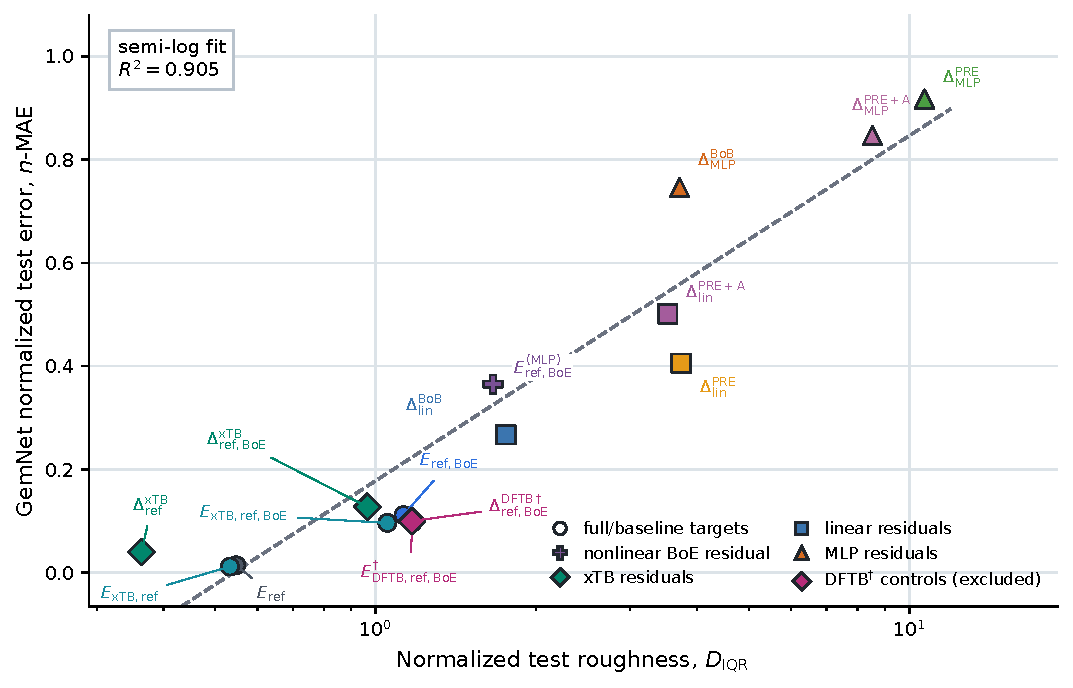
\includegraphics[width=0.90\linewidth]{fig04_roughness_nmae}
  \caption{\textbf{Model-relative roughness and normalized GemNet test error.} Mean GemNet test \(n\)-MAE, defined as \(\operatorname{MAE}_{\rm test}/\operatorname{IQR}_{\rm test}(y)\), is plotted against test \(D_{\rm IQR}\) for 13 primary targets. Roughness is measured on the standardized test PRE+A graph, and the horizontal axis is logarithmic. Marker shapes identify the target classes shown in the legend. Points show means across three GNN seeds. The dashed line is the semi-log regression over the 13 primary target means (\(R^2=0.905\)). Magenta DFTB\(^\dagger\) points are single-seed, valid-subset controls, excluded from the regression and correlations.}
  \label{fig:roughness-nmae}
\end{figure}

Across these primary targets, GemNet's normalized test error increases approximately linearly with \(\log D_{\rm IQR}\), yielding \(R^2=0.905\) in PRE+A space (Fig.~\ref{fig:roughness-nmae}). SchNet exhibits a corresponding association in PRE space (\(R^2=0.946\); SI Note~6). Practically, targets that vary more sharply between structurally similar molecules tend to be harder for downstream GNNs to learn relative to their spread. Leave-one-target-out sensitivity checks show that this trend is not driven by any single target, maintaining \(R^2\in[0.872,0.927]\) for GemNet and \(R^2\in[0.927,0.965]\) for SchNet (SI Note~7). These ranges describe refitted associations, not cross-validated prediction scores.

Because \(D_{\rm IQR}\) and \(n\)-MAE share target IQR as a scaling factor, their correlation may partly reflect shared-denominator normalization.\cite{pearson1897spurious} We conducted sensitivity controls to assess the contribution of molecular-neighbourhood alignment beyond this coupling. Removing IQR normalization from both axes reduces \(R^2\) to 0.019 for GemNet and 0.067 for SchNet, showing that the strong normalized association does not extend to the relationship between log raw roughness and absolute test error (SI Note~7).

To assess the contribution of label alignment with molecular graph geometry, we performed 5,000 joint-label permutations (SI Note~7). Shuffling target values across molecules preserves target distributions and IQRs while severing their connection to chemical structure; graphs and GNN test errors remain fixed. Although target distributions and normalization sustain a high shuffled correlation (median \(R^2=0.862\) for GemNet and 0.855 for SchNet), the observed positive correlation exceeds every shuffled result for both models (one-sided \(p\approx0.00020\), using the plus-one correction;\cite{phipson2010permutation} SI Note~7). Furthermore, among all three target pairs whose IQRs differed by at most 10\%, the smoother target also had the lower mean normalized test error for both SchNet and GemNet (SI Note~7).

Together, these results support architecture-aligned target roughness (\(D_{\rm IQR}\)) as a scale-invariant candidate pre-training diagnostic of relative target learnability. Molecular-neighbourhood alignment contributes information beyond the shuffled target-distribution baseline, although normalization contributes substantially to the observed association. These retrospective results do not establish a causal mechanism or guarantee predictive performance for new target families.

\subsection{Target design controls out-of-domain transfer}
\label{sec:ood-transfer}

To evaluate whether favourable target design enhances transferability beyond the training distribution, we tested model predictions on the QM9 dataset \cite{ramakrishnan2014quantum}. While QM9 shares elements with tmQM, it shifts the chemical domain from transition-metal complexes to small organic molecules, altering molecular size, bonding motifs, and coordination environments. To isolate this chemical domain shift from discrepancies in electronic-structure fidelity, QM9 DFT reference energies were recomputed at the identical level of theory used for tmQM, with transformed targets generated using frozen, train-only baseline parameters (SI Methods).

Evaluating out-of-domain (OOD) performance across distinct chemical families can introduce systematic dataset-level energy offsets due to divergent stoichiometry and size distributions. Because raw OOD MAE combines these global offsets with molecule-to-molecule errors, we assessed trend preservation using two complementary metrics: Kendall rank correlation (\(\tau\)), which quantifies energetic ordering, and mean-shifted MAE, which measures residual scatter after removing a single dataset-wide offset (SI Note~5). This offset is estimated from the QM9 reference labels, rendering mean-shifted MAE an oracle diagnostic rather than an independently calibrated prediction score. All reconstructed routes were mapped back onto the parent DFT-BoE energy target prior to comparison.

\begin{figure}[H]
  \centering
  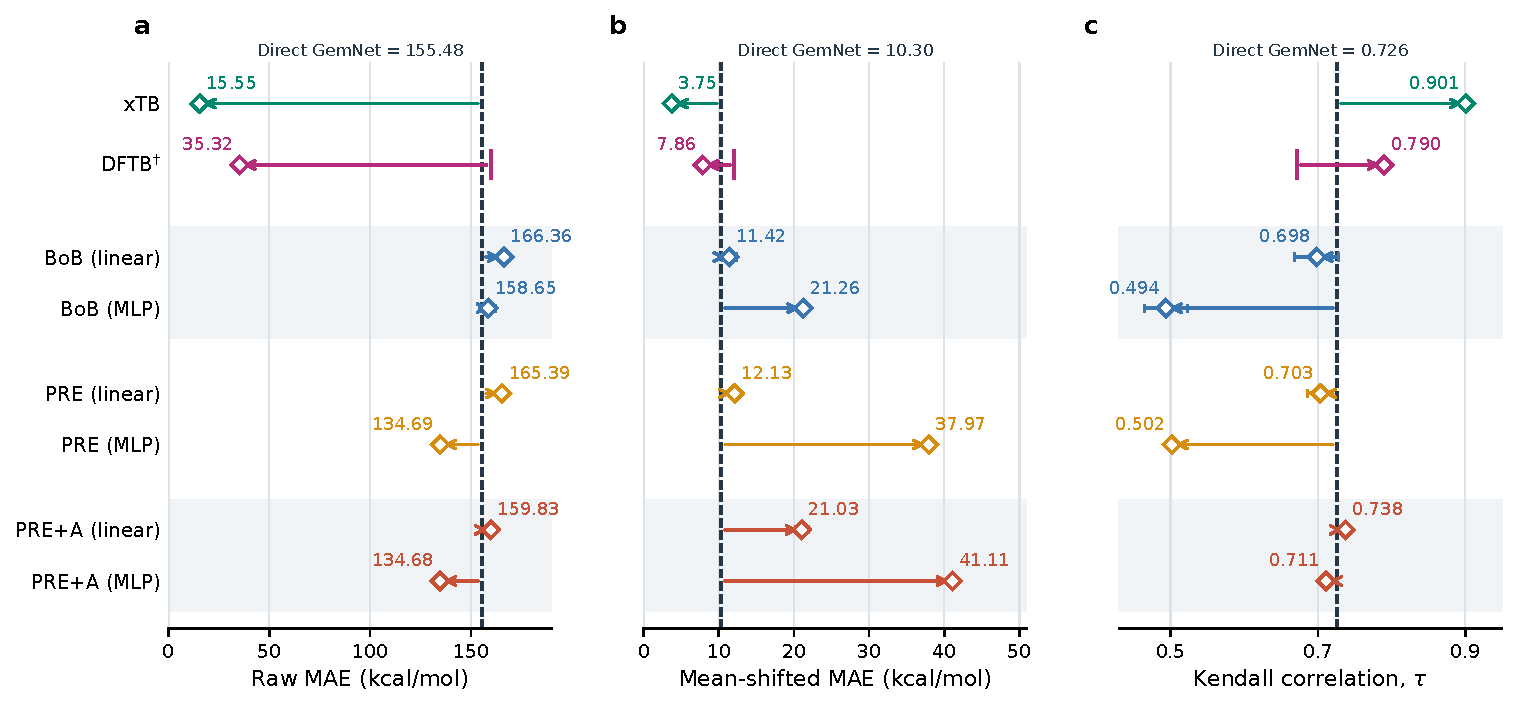
\includegraphics[width=\linewidth]{fig03_qm9_transfer}
  \caption{\textbf{Out-of-domain GemNet transfer from tmQM to QM9.} \textbf{a,} Raw MAE. \textbf{b,} Mean-shifted MAE using one offset estimated from QM9 labels. \textbf{c,} Kendall correlation. Diamonds show baseline-plus-GemNet predictions against \(E_{\rm ref,BoE}\); dashed lines mark direct GemNet. Primary results are three-seed means with sample-SD bars on 128,988 common molecules. Magenta DFTB\(^\dagger\) is a seed-101 control on 128,978 valid molecules; its short reference ticks and arrows use direct seed 101 on the same subset (SI Notes~5 and 8).}
  \label{fig:qm9-transfer}
\end{figure}

Among all primary GemNet routes evaluated on QM9, the composition-referenced xTB residual achieved the best mean transfer performance across the three reported metrics (Fig.~\ref{fig:qm9-transfer}). Learning on the xTB residual reduced mean-shifted MAE from \(0.01641\)~Ha for direct GemNet to \(0.00598\)~Ha while increasing Kendall \(\tau\) from \(0.726\) to \(0.901\) (Fig.~\ref{fig:qm9-transfer}b,c). It also yielded the lowest raw MAE, reducing error from \(0.2478\) to \(0.0248\)~Ha (Fig.~\ref{fig:qm9-transfer}a), showing that its transfer advantage does not rely on mean-shift offset calibration. In contrast, no local descriptor baseline improved upon direct GemNet on both trend metrics; linear PRE+A slightly increased mean Kendall correlation (\(\tau=0.738\)) but increased mean-shifted MAE to \(0.03351\)~Ha (Fig.~\ref{fig:qm9-transfer}b,c). Furthermore, GemNet preserved the ordering of the predicted xTB residual itself (\(\tau=0.789\) on the common QM9 cohort), supporting transfer of the learned residual correction rather than only the reconstructed energy ranking (SI Note~5). SchNet exhibited parallel improvements on the xTB residual, reducing mean-shifted MAE from \(0.01563\) to \(0.00665\)~Ha and increasing Kendall \(\tau\) from \(0.746\) to \(0.895\) (SI Note~5).

Semiempirical density-functional tight-binding (DFTB\(^\dagger\)) provided supporting evidence on its valid subset, reducing raw MAE from \(0.2547\) to \(0.0563\)~Ha, reducing mean-shifted MAE from \(0.01917\) to \(0.01253\)~Ha, and increasing Kendall \(\tau\) from \(0.671\) to \(0.790\) relative to matched-subset direct GemNet (SI Notes~5 and 8). This seed-101 control uses a different training subset and does not provide a three-seed uncertainty estimate.

These results motivate the principle of \textbf{baseline complementarity} in physical target design. Baselines constructed from local geometric descriptors share information with message-passing GNNs and may remove smooth variations that message-passing layers naturally learn while leaving behind residuals that are rough relative to their scale. In contrast, semiempirical quantum methods supply molecule-wide electronic-structure priors---including interactions beyond standard spatial cutoffs---that may complement downstream neural architectures. Tu and Rowley demonstrated such complementarity for long-range interactions, showing that a DFTB3 baseline supplies intermolecular interactions beyond a local neural network's cutoff and improves transferability over direct learning \cite{tu2026transferable}. While target scale and representation smoothness provide complementary diagnostics rather than strict guarantees for transfer, combining semiempirical physical baselines with architecture-aligned GNNs improves out-of-domain generalization in the present comparisons; the specific physical mechanism remains unresolved.
